\DiaryEntry{BJT Switch}{2017-03-19}{Circuits}

The following circuit is taken from the Art of Electroncis, Fig 2.10.

Conventions: The current through a resistor $R_x$ is denoted by $I_x$.

\begin{figure}[htb]
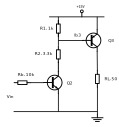
\includegraphics[scale=0.5]{images/switch_2_bjt.png}
\end{figure}

\subsection{Analysis}

\paragraph{Q2 closed - $V_\text{in} = 0V$}: Q2 is open and its collector at a voltage of 15V. The base of Q3 is also at 15V and therefore Q3 is off. Its emitter is at zero voltage and the current through $R_L$ is zero.

\paragraph{Q2 opened - $V_\text{in} = 3V$}: Q2 opens, the voltage at its collector is $\approx 0V$. The collector current of Q2 is therefore

\bee
\frac{(15-0.6)V}{3.3k\Omega} \approx 4.4mA
\eee
%
Therefore the base current of Q2 is estimated with $4.4mA / 25 \approx 180\mu A$ (with an estimated current gain of 25). This requires a base resistor $R_b$ of about $3V/180\mu A \approx 17k\Omega$. We took $10k\Omega$ to ensure Q2 is deeply saturated.

The $4.4mA$ from above are driven by two sources: (i) Via $R_1$, but note that this current is only about $0.6V / 1k\Omega \approx 0.6mA$ (because Q3 is open, its base is $\approx 0.6V$ \emph{lower} than its emitter - this is a PNP transistor!), and (ii) from the base of Q3 which therefore must be $4.4mA - 0.6mA \approx 3.8mA$.
%
Since Q3 is open, its emitter of Q3 is at $\approx 15V$ as Q3 is open and the current through $R_L$ is about $15V / 50\Omega \approx 300mA$.


\subsection{Simulation}

The following ngspice netlist describes the circuit from above.

\begin{verbatim}

.model mnpn npn is=1e-16
.model mpnp pnp is=1e-16

vcc vplus gnd dc 15V
vin in gnd dc 3V

*   C   B   E
q2 q2c q2b gnd    mnpn
q3 rl  q3b vplus  mpnp

Rb in q2b 10kOhm

R1 vplus q3b    1kOhm
R2 q3b q2c 3.3kOhm

Rload gnd rl 50Ohm

.end
\end{verbatim}

It can be loaded into ngspice by (i) starting ngspice with the netlist filename as parameter, or (ii) inside ngspice with \verb! source <filename>!.

Simulating the operating point can be triggered with \verb op (and changing the vin voltage). Voltages can then be printed via \verb! print v(<node>)!; e.g. \verb! print v(q3b)! yields $14.1V$. A \verb show shows information about the bipolar transistors; we see that the B-E voltage of Q3 is $\approx 0.9V$ (and not $0.6V$ as used above).

However, simulation does not provide information about other currents; e.g. through resistors. We therefore need to add voltage sources (with zero voltage) in series whereever we want to measure a current.

The netlist therefore looks as follows (with vr1, vr2, and vrload being such dummy voltage sources).

\begin{verbatim}

.model mnpn npn is=1e-16
.model mpnp pnp is=1e-16

vcc vplus gnd dc 15V
vin in gnd dc 3V

*   C   B   E
q2 q2c q2b gnd    mnpn
q3 rl  q3b vplus  mpnp

Rb in q2b 10kOhm

R1 vplus r1temp    1kOhm
R2 q3b r2temp 3.3kOhm

vr1 r1temp q3b dc 0V
vr2 r2temp q2c dc 0V
vrload rl rltemp dc 0V

Rload gnd rltemp 50Ohm

.end

\end{verbatim}

Issuing \verb!show! now displays the required currents. It shows - e.g. - that the current through $R_2$ is $\approx 4.24mA$.


\paragraph{DC Sweep.} Finally, we want to sweep the input voltage and display the emitter voltage of Q3 as function of the input voltage. To this end, we include the line \verb!.dc vin 0 2 0.01! towards the end of the netlist file. After (re)loading, we can run the simulation with \verb!run!. Either we plot the thing directly in ngspice \verb!plot v(rl)! or we export the data as table \verb!wrdata rl_voltage rl! and plot it via Julia.

The following plot shows the result: The threshold is at $\approx 1V$ and quite steep (from $0.8V$ to $1.2V$).

\begin{figure}[htb]
\includegraphics[scale=0.5]{images/rl_voltage.png}
\end{figure}




